

%Dati il layout di una metropolitana e la tabella orario dei treni che si vogliono far circolare. Viene definito il modello delle missioni dei singoli treni. Il modello delle missioni unito al modello dello stato della linea formano il modello di scheduling del sistema. 
%Il risultato dell'analisi del model chec ker 

%In questo paragrafo noi descriviamo l'approccio utilizzato per verificare ed eliminare i deadlock in una metropolitana.
%In particolare questa è l'analisi fatta dall'ATS per schedulare i treni in caso di ritardo senza generare deadlock.

In this section we describe the approach used to verify and delete deadlock in a subway.
In particular, this is the analysis performed by the ATS to schedule trains in case of delay without generating deadlocks.

%Il nostro approccio si basa sull'utilizzo iterativo di un model checker per verificare la presenza di deadlock di una metropolitana.

Our approach is based on an iterative model checker to verify the presence of deadlocks of a subway.

\begin{figure}[h!]
	\begin{centering}	
	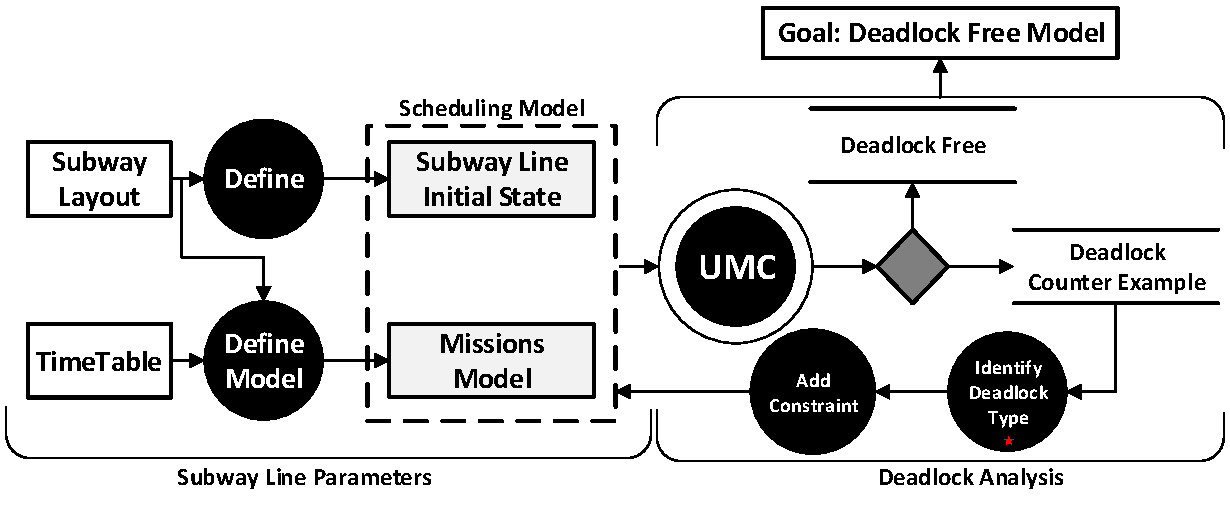
\includegraphics[width=0.45\textwidth, clip]{img/processo}
	\caption{Overview of the approach}
	\label{fig:process}
	\end{centering}
\end{figure}

%La figura~\ref{fig:process} descrive graficamente l'approccio usato.
The figure ~\ref{fig:process} describes the approach used.

%%Nella prima fase, che chiamiamo SLP, vengo preparati i dati per effettuare l'analisi di deadlock della linea.
%I dati di partenza sono  il layout della metropolitana e la tabella orario dei treni che si vogliono far circolare. Questi dati sono usati per definire i modelli delle missioni dei singoli treni. 

The source data are the subway  layout and the metro timetable. Both are used to define models of the missions of individual trains, see figure~\ref{fig:lmissionm}.


%Invece il layout della metropolitana viene usato anche per definire lo stato iniziale della linea. Cosi è possibile bloccare alcuni tratti di metropolitana perchè impegnati ad esempio da lavori di manutenzione.

Whereas the layout of the subway is also used to define the initial state of the line, see figure~\ref{fig:lstateline}. So you can lock some parts of the subway because it involved such as maintenance or insert the initial position of train.

%I modelli di missione e lo stato iniziale della metropolitana costituiscono il modello di scheduling della metropolitana.

The models of the mission and the model initial state of the subway they represent the model of scheduling of the subway, see figure~\ref{fig:SchedulingModel}.

%Il modello di scheduling viene analizzato tramite il model checker UMC[inserire riferimento]
The scheduling model is analyzed using the model checker UMC [insert reference]
%UMC permette di specificare come un insime di statecharts UML e di verificare proprità relative all'evoluzione del sistema. 
UMC allows to specify a system as a set of UML Statecharts and verify properties related to the evolution of the system.

%Se risultato del modelchecker è controesempio di deadlock. Si identificano i pattern di deadlock e si inserisco delle nuove regole nelle aree scritiche identificate. Altrimenti potremo affermare che il modello è libero di deadlock.

If the result of the model checker is deadlock counter example we identify patterns of deadlocks and insert the new contraints in the critical areas identified, see section~\ref{sec:deadlockpatterndefinition}. Otherwise, we can conclude that the model is free of deadlocks. 
%Quindi tutti i treni sono ingrado di arrivare a destinazione senza generare deadlock.
So all the trains, present into timetable, are able to arrive at your destination without generating deadlock.